\section{区域积分}
\label{sec:multivariable-region-integration}

平面薄片的质量由面密度在整块区域上的累计给出，空间物体的质量则要累计体密度。
这里的被积对象都是多元标量函数$f:D\subseteq\mathbb R^d\to\mathbb R$：输入有多个坐标，每个位置只输出一个待累计的数。
一元积分的长度权重需要相应换成$d$维勒贝格测度，积分的简单函数构造和绝对可积要求则继续适用。

实际计算还要回答两个问题：何时能逐个坐标做一元积分，何时能改用另一套坐标？
前者需要非负性或绝对可积性来保证累次积分成立，后者需要坐标变换的Jacobian来校正体积。
坐标变换是一个向量值映射，不是这里的标量被积函数。
最后再把被积函数看成依赖参数的一族标量函数，讨论积分的连续性和求导。切片与坐标计算可参考\scite{math-openstax-calculus3}。

\subsection{多维测度与乘积测度}
\label{sec:comb-multidimensional-product-measure}

实轴上的测量建立以后，还需要测量成对或多坐标对象构成的集合。
有限集合满足$|A\times B|=|A||B|$，长方形满足“面积等于两边长度之积”，这提示我们用各方向测度的乘积测量矩形。
下面先把区间覆盖构造直接推广到多维，再说明一般测度空间中的乘积构造；两者会在多维长度、面积和体积上衔接。

\subsubsection{多维勒贝格测度}

\paragraph{坐标盒}

$d$维坐标盒是区间的笛卡尔积，例如
\[
 Q=\prod_{i=1}^d(a_i,b_i),\qquad a_i<b_i.
\]
它的体积为$\prod_i(b_i-a_i)$。例如$(0,2)\times(0,3)$的面积为$6$。
所有开盒生成$\mathbb R^d$上的Borel $\sigma$代数$\mathcal B(\mathbb R^d)$。

\paragraph{多维勒贝格测度}

一维外测度通过可数区间覆盖比较总长度。把覆盖对象改为开盒、长度改为体积，就能用同一思路测量$\mathbb R^d$中的集合：
\[
 m_d^*(E)=\inf_{\substack{E\subseteq\bigcup_{n=1}^{\infty}Q_n\\
 Q_n\text{为开坐标盒}}}\sum_{n=1}^{\infty}\operatorname{vol}(Q_n).
\]
下确界取遍$E$的所有可数开盒覆盖。再要求集合$A$对每个测试集合$E\subseteq\mathbb R^d$满足
$m_d^*(E)=m_d^*(E\cap A)+m_d^*(E\setminus A)$，就得到勒贝格可测集族$\mathcal L_d$。
外测度限制在这个$\sigma$代数上，给出完备的$d$维勒贝格测度$m_d$，其中$m_1=m$。
前面关于外测度、可测分割和可数可加性的论证只需将区间换成盒，即可按同样步骤推广；$m_d$为坐标盒赋予边长之积。

每个欧氏开集都是其中有理端点开盒的可数并，所以开盒生成的Borel范围包含全部开集。
因此$\mathcal B(\mathbb R^d)\subseteq\mathcal L_d$；勒贝格范围还包含Borel零测集的全部子集。

\subsubsection{乘积测度}

多维勒贝格测度使用欧氏空间中的坐标盒；一般的乘积测度则从任意两个测度空间出发，以$A\times B$作为基本矩形。
为保证下面的乘积测度存在且唯一，先说明所采用的$\sigma$有限条件：允许总量无限，但空间能够被可数个有限测度部分覆盖。

\paragraph{$\sigma$有限测度}

若整个空间测度有限，就称为有限测度。更一般地，可要求空间由可数个有限测度集合覆盖。
\begin{definition}[$\sigma$有限测度]
\label{def:analysis-sigma-finite-measure}
若存在$E_n\in\mathcal A$，使$X=\bigcup_{n=1}^{\infty}E_n$且每个$n$都满足$\mu(E_n)<\infty$，称测度空间$(X,\mathcal A,\mu)$为\term{$\sigma$有限}（sigma-finite）的。
\end{definition}

例如$\mathbb R=\bigcup_n[-n,n]$，每段长度有限，所以勒贝格测度$\sigma$有限。
有限集合上的计数测度是有限测度；可数无限集合上的计数测度虽总量无限，仍$\sigma$有限。
不可数集合上的计数测度则不$\sigma$有限，因为有限测度子集只能有限，可数个这样的集合仍不能覆盖不可数集。

\paragraph{乘积$\sigma$代数}

矩形适合规定基本赋值，但矩形的并或补一般不再是一个矩形，因此不能只把矩形本身当作全部可测集合。
设$(X,\mathcal A)$、$(Y,\mathcal B)$为可测空间。包含全部矩形$A\times B$
（$A\in\mathcal A,B\in\mathcal B$）的最小$\sigma$代数称为乘积$\sigma$代数，记为$\mathcal A\otimes\mathcal B$。
例如两个有限集合都采用全部子集时，每个网格单点都是矩形，乘积范围也是全部网格子集。

\paragraph{乘积测度}

在两个空间上分别规定测度后，还要为成对对象赋予联合的大小。对可测矩形，所需规则是把两个方向的测度相乘。

\begin{definition}[乘积测度]
\label{def:analysis-product-measure}
设$(X,\mathcal A,\mu)$、$(Y,\mathcal B,\nu)$为$\sigma$有限测度空间。
在$\mathcal A\otimes\mathcal B$上满足
\begin{equation}
 (\mu\otimes\nu)(A\times B)=\mu(A)\nu(B)
 \label{eq:comb-product-measure-rectangle}
\end{equation}
的测度称为\term{乘积测度}（product measure），记为$\mu\otimes\nu$，其中约定$0\cdot\infty=0$。
\end{definition}

定义规定了矩形应有的测度，还需要确认这个规定能够一致扩展到整个乘积$\sigma$代数。$\sigma$有限条件使这一扩展既存在又唯一。
\begin{theorem}[乘积测度的存在唯一性]
若$(X,\mathcal A,\mu)$与$(Y,\mathcal B,\nu)$均为$\sigma$有限测度空间，则存在唯一的测度$\mu\otimes\nu$定义在$\mathcal A\otimes\mathcal B$上，并满足式~\eqref{eq:comb-product-measure-rectangle}。
\end{theorem}
这里引用该扩展定理，完整证明可参考测度论教材\scite{math-folland1999real}。
例如$X=\{x_1,x_2\}$的点权重为$1,2$，$Y=\{y_1,y_2\}$的点权重为$3,4$，
则四个网格点的权重分别为$3,4,6,8$，总权重$21=(1+2)(3+4)$。
一般有限网格满足
\[
 (\mu\otimes\nu)(E)=\sum_{(i,j):(x_i,y_j)\in E}u_iv_j,
\]
其中$u_i,v_j$为两侧的点权重；矩形公式正是有限分配律。


图~\ref{fig:analysis-process-product-measure-grid}将这组点权重画成矩形网格，使矩形赋值的乘法与全部累计的加法对应起来。
\begin{figure}[!htbp]
 \centering
 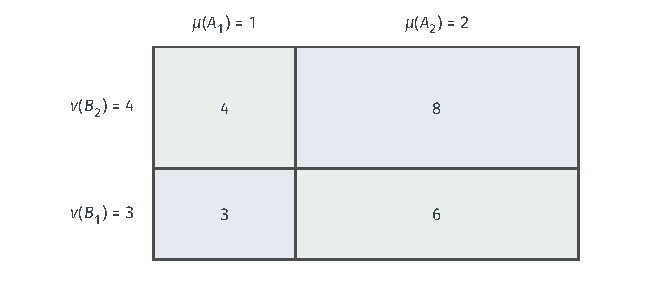
\includegraphics[width=112mm]{figures/01-mathematical-preliminaries-upper/01-mathematical-language-combinatorics-analysis-optimization/tikz/chapter3-concept-processes/product-measure-grid.pdf}
 \caption{列权重为$1,2$，行权重为$3,4$，四个格子的乘积权重为$3,6,4,8$，总量$21$。列宽及行高分别按各自权重成比例，因此面积也按乘积成比例；这些是有限原子空间的权重，不是任意二维分布都必须满足的关系。}
 \label{fig:analysis-process-product-measure-grid}
\end{figure}

\paragraph{欧氏乘积与完备化}

前面分别从欧氏盒和一般矩形构造可测范围，现在核对这两条路线在欧氏空间是否一致。
欧氏空间的Borel范围满足
\begin{equation}
 \mathcal B(\mathbb R^p)\otimes\mathcal B(\mathbb R^q)=\mathcal B(\mathbb R^{p+q}).
 \label{eq:comb-borel-product-structure}
\end{equation}
开盒是低维Borel集合的矩形，给出一个方向的包含。
反过来，坐标投影对低维开盒的原像可写成可数个高维有界开盒的并，因而是Borel集合。
原像保持补集、可数并，这项结论扩展到全部低维Borel集合；
两个投影原像相交便给出Borel矩形，得到另一方向的包含。

把$m_p,m_q$限制在各自Borel范围上，它们的乘积在开盒上给出体积，
由$\sigma$有限唯一扩展，等于Borel范围上的$m_{p+q}$。
再作完备化才得到完备的多维勒贝格测度空间。
即使两个因子测度完备，乘积范围也未必完备，所以应说明采用乘积$\sigma$代数还是其完备化。
函数的累次积分在本节后面讨论，矩形赋值公式还不能单独推出积分换序。


\subsection{区域积分的定义与可积性}
\label{sec:multivariable-riemann-lebesgue}

测度确定区域有多大，被积函数确定各位置贡献多少。现在把一元可测函数与勒贝格积分的定义搬到$\mathbb R^d$上，明确改变的是输入空间，而不是积分的构造方法。

\subsubsection{多元可测函数}

要累计各个函数值对应的区域，首先必须能测量这些区域。与一元情形一样，检查所有阈值以上的原像集合就足够了。
\begin{definition}[多元可测函数]
设$D\in\mathcal L_d$。函数$f:D\to\overline{\mathbb R}$称为勒贝格可测函数，是指对每个$a\in\mathbb R$，集合
\[
 \{\bm x\in D:f(\bm x)>a\}
\]
都属于$\mathcal L_d$。
\end{definition}

连续标量函数的开集原像相对于$D$开，而相对开集可写为$D$与一个欧氏开集的交，因此可测。
连续性仍是可测性的充分条件；例如$\mathbb I_{\mathbb Q^d}$处处不连续，却是可测函数，因为$\mathbb Q^d$可数。
这里没有要求函数输出向量；向量值函数的分量可测性不参与本节区域积分的定义。

\subsubsection{区域积分的定义}

\paragraph{非负标量函数的积分}

先累计非负贡献，就不会遇到正负无穷相消。可测简单函数在每个可测小块上取常值，其积分等于常值乘该块测度再求和；一般非负函数仍由下方的简单函数逼近。
\begin{definition}[非负区域积分]
设$D\in\mathcal L_d$，$f:D\to[0,\infty]$可测。定义
\[
 \int_D f\,\mathrm dm_d
 =\sup_{\substack{0\leq s\leq f\\s\text{为可测简单函数}}}
 \int_D s\,\mathrm dm_d.
\]
若$s=\sum_{j=1}^n c_j\mathbb I_{E_j}$，其中$E_j\subseteq D$可测、两两不交且$c_j\geq0$，则$\int_Ds\,\mathrm dm_d=\sum_jc_jm_d(E_j)$，约定$0\cdot\infty=0$。
\end{definition}

这个积分可以取$+\infty$。在全空间上把$f$作零延拓，就有
$\int_Df\,\mathrm dm_d=\int_{\mathbb R^d}f\mathbb I_D\,\mathrm dm_d$；这里的乘积表示区域外取零。
区域不必是矩形，定义也不要求它的边界零测。

\paragraph{有符号标量函数的积分}

函数可以取正负值时，仍应先分别累计正负贡献。为了得到可以作普通加减的有限积分，本章继续要求绝对值的总贡献有限。
\begin{definition}[区域上的勒贝格可积性]
设$D\in\mathcal L_d$，$f:D\to\overline{\mathbb R}$可测。若
\begin{equation}
 \int_D|f|\,\mathrm dm_d<\infty,
 \label{eq:multivariable-lebesgue-integrability}
\end{equation}
称$f$在$D$上勒贝格可积，并定义
\[
 \int_Df\,\mathrm dm_d=\int_Df^+\,\mathrm dm_d-\int_Df^-\,\mathrm dm_d.
\]
\end{definition}

绝对可积性保证正负部分的积分都有限，也保证$f$几乎处处为有限值。
在零测例外集上把无穷值改成零，不改变积分。若正负部分的积分都为无穷，则不能用两者相减定义勒贝格积分。
例如$\mathbb I_{\mathbb Q^d}$在单位长方体上的积分为零，因为可数集的$d$维测度为零。

\paragraph{二重积分与多重积分}

二维时把上述积分写为
\[
 \iint_Df(x,y)\,\mathrm dx\,\mathrm dy=\int_Df\,\mathrm dm_2;
\]
三维中常记为$\iiint_Df\,\mathrm dV$；$d$维时统一写作
\[
 \int_Df(\bm x)\,\mathrm d\bm x=\int_Df\,\mathrm dm_d.
\]
“二重”或“多重”表示输入维数，并不表示已经选择了逐坐标的计算次序。
例如$f\equiv3$、$D=[0,1]\times[0,2]$时，积分为$3m_2(D)=6$。
函数值在小块上近似常数时，该块贡献近似等于函数值乘面积；这是简单函数累计的几何解释。

\subsubsection{可积性的判别}

\paragraph{有限测度区域上的有界函数}

若$m_d(D)<\infty$，$f$可测且$|f|\leq M<\infty$几乎处处成立，则
\[
 \int_D|f|\,\mathrm dm_d\leq M m_d(D)<\infty.
\]
因此连续函数在紧长方体上可积，更一般地，在任意有限测度区域上有界的可测函数也可积。
无界函数仍可能可积，而无限体积区域上的有界函数未必可积；所检查的始终是绝对值的总累计。

\paragraph{可积控制函数}

若存在非负可积函数$H$使$|f|\leq H$几乎处处成立，则比较不等式给出$\int_D|f|\leq\int_DH<\infty$，从而$f$可积。
这把无界函数的判别转为寻找一个总量有限的上界。后面的非负累次积分还会提供直接计算$\int_D|f|$的方法。

\paragraph{递增区域上的截断}

若$D_n\uparrow D$且各$D_n$可测，单调收敛给出
\[
 \int_D|f|\,\mathrm dm_d
 =\lim_{n\to\infty}\int_{D_n}|f|\,\mathrm dm_d.
\]
因此右侧有有限上界当且仅当$f$可积；可积时，支配收敛又给出$\int_{D_n}f\to\int_Df$。
这样得到的积分值不依赖所选递增覆盖。缺少绝对可积性时，沿某种截断区域得到的正负相消极限，不能替代这里的有限有符号积分。

\subsection{区域积分的基本性质}

多维区域积分仍是测度空间上的勒贝格积分，前面已证明的性质可直接使用。下面固定可测区域$D$，各有符号公式均要求所列函数在相应区域上绝对可积，微元统一写为$\mathrm dm_d$。

\paragraph{加法}

若$f,g$在$D$上可积，则$f+g$也可积，且
\[
 \int_D(f+g)\,\mathrm dm_d=\int_Df\,\mathrm dm_d+\int_Dg\,\mathrm dm_d.
\]
绝对可积性由$|f+g|\leq|f|+|g|$保证，相加公式由一般勒贝格积分的线性给出。

\paragraph{减法}

对同一组可积函数，有
\[
 \int_D(f-g)\,\mathrm dm_d=\int_Df\,\mathrm dm_d-\int_Dg\,\mathrm dm_d.
\]
这里两项都是有限数，因此不会出现无穷减无穷。

\paragraph{常数倍}

若$c\in\mathbb R$且$f$在$D$上可积，则$cf$可积，并满足
\[
 \int_Dcf\,\mathrm dm_d=c\int_Df\,\mathrm dm_d.
\]
系数只改变各位置的标量贡献，不改变积分区域及其测度。

\paragraph{区域可加性}

若$f$在两两不交的可测集合$D_j$之并上可积，则
\[
 \int_{\bigcup_jD_j}f\,\mathrm dm_d=\sum_j\int_{D_j}f\,\mathrm dm_d.
\]
有限并直接来自指示函数的分解，可数并使用一般积分的区域可加性；绝对可积性保证右侧级数绝对收敛。
两块区域允许重叠时，只需扣除被重复计入的交集：
\[
 \int_{A\cup B}f\,\mathrm dm_d
 =\int_Af\,\mathrm dm_d+\int_Bf\,\mathrm dm_d-\int_{A\cap B}f\,\mathrm dm_d.
\]
这由$\mathbb I_{A\cup B}=\mathbb I_A+\mathbb I_B-\mathbb I_{A\cap B}$得到。公共边界零测的有限区域分割，是重叠部分不影响积分的常见情形。

\paragraph{单调性}

若$f\leq g$几乎处处成立，则
\[
 \int_Df\,\mathrm dm_d\leq\int_Dg\,\mathrm dm_d.
\]
特别地，$0\leq f\leq M$且$m_d(D)<\infty$时，有$0\leq\int_Df\leq M m_d(D)$。这也给出忽略一小块区域时的误差上界。

\paragraph{绝对值不等式}

可积函数满足
\[
 \left|\int_Df\,\mathrm dm_d\right|\leq\int_D|f|\,\mathrm dm_d.
\]
它来自$-|f|\leq f\leq|f|$和积分单调性。由于零测集贡献为零，上述所有结论都允许在零测集上修改有限函数值；测度的完备性保证这种修改保持可测。

\subsection{累次积分}
\label{sec:multivariable-iterated-integrals}

直接累计整个区域往往不便计算。固定一个坐标以后，剩下的函数是低一维的截面；先积分这些截面，再累计外层坐标，就得到累次积分。它何时等于区域积分，需要检查非负性或绝对可积性，而不是只交换微分记号。

\subsubsection{截面与累次积分}

对$f:X\times Y\to\overline{\mathbb R}$，固定$x$所得函数$f_x(y)=f(x,y)$称为关于$y$的截面。
若各截面的积分有意义，外层积分也有意义，则
\[
 \int_X\left(\int_Yf(x,y)\,\mathrm d\nu(y)\right)\mathrm d\mu(x)
\]
称为先对$y$、再对$x$的累次积分。反向次序需要另行检查，并不能由这个记号本身推出两者相等。

有限网格上的这种计算就是先求每行加权和，再求行与行之间的加权和；一般乘积测度将同一问题扩展到连续坐标。
乘积测度是一种特定的联合权重构造，一般二元概率分布不必等于两边概率测度的乘积；联合分布与独立性的进一步讨论可参考\BookChapterRef{chap:probability-theory}{卷2《数学准备：概率、因果与决策》的“随机变量与概率基础”章}。

\subsubsection{累次积分的成立条件}

下面固定两个$\sigma$有限测度空间$(X,\mathcal A,\mu)$与$(Y,\mathcal B,\nu)$，先对乘积$\sigma$代数上的可测函数给出结论。
在这个可测范围内，每个截面都可测。若两个因子空间均完备，而函数只对乘积测度的完备化可测，则截面只保证几乎处处可测。若因子尚未完备，应先对因子作完备化，再使用这一表述。

\paragraph{非负可测函数的累次积分}

非负贡献不会因相消而改变总量，因此允许总积分为无穷。Tonelli定理把这一事实精确地表述为两个累次积分与乘积空间积分相等。
\begin{theorem}[Tonelli定理]
\label{thm:analysis-tonelli-fubini}
设$f:X\times Y\to[0,\infty]$对$\mathcal A\otimes\mathcal B$可测。每个截面都可测，两个内层积分函数
\[
 x\longmapsto\int_Yf(x,y)\,\mathrm d\nu(y),\qquad
 y\longmapsto\int_Xf(x,y)\,\mathrm d\mu(x)
\]
也分别可测，且
\[
 \begin{aligned}
 \int_{X\times Y}f\,\mathrm d(\mu\otimes\nu)
 &=\int_X\left(\int_Yf(x,y)\,\mathrm d\nu(y)\right)\mathrm d\mu(x)\\
 &=\int_Y\left(\int_Xf(x,y)\,\mathrm d\mu(x)\right)\mathrm d\nu(y).
 \end{aligned}
\]
三个积分允许共同取$+\infty$。若两个因子空间均完备，函数只对乘积测度的完备化可测，上述等式仍成立，但截面可测性以及内层积分函数的定义都只要求几乎处处成立。
\end{theorem}

\paragraph{绝对可积函数的累次积分}

有符号函数不能只依靠逐行或逐列的有限值来保证换序。先对$|f|$应用非负版本，确认整个乘积空间上的绝对贡献有限，就能排除正负无穷相消。
\begin{theorem}[Fubini定理]
\label{thm:analysis-fubini-integrable}
设$f:X\times Y\to\overline{\mathbb R}$对$\mathcal A\otimes\mathcal B$可测，并满足
$\int_{X\times Y}|f|\,\mathrm d(\mu\otimes\nu)<\infty$。
则$f_x$对几乎每个$x$可积，另一方向的截面也对几乎每个$y$可积。
把内层积分函数在相应例外集上置为零后，它们分别可积，并且
\[
 \begin{aligned}
 \int_{X\times Y}f\,\mathrm d(\mu\otimes\nu)
 &=\int_X\left(\int_Yf(x,y)\,\mathrm d\nu(y)\right)\mathrm d\mu(x)\\
 &=\int_Y\left(\int_Xf(x,y)\,\mathrm d\mu(x)\right)\mathrm d\nu(y).
 \end{aligned}
\]
三个积分都是有限值。若两个因子空间均完备，$f$只对乘积测度的完备化可测，结论仍成立，但截面的可测性和可积性均只作几乎处处的断言。
\end{theorem}

若$f$在零测集上取无穷值，可先将那些值改成零再处理有符号积分。事实上，$N=\{|f|=\infty\}$满足$|f|\geq M\mathbb I_N$对所有$M>0$成立，绝对积分有限强制$N$零测；改值不影响积分。

证明可分为集合与函数两层。对矩形指示函数$\mathbb I_{A\times B}$，三种积分都等于
$\mu(A)\nu(B)$；有限可加性把这个结论扩展到有限分割形成的集合。
从这些集合进入乘积$\sigma$代数中的\emph{任意}可测集合，还需要测度论的扩张论证，
不是仅靠每个矩形上的等式便能完成；完整论证见所引测度论教材
\scite{math-folland1999real}。
本章关注扩张之后的函数层：指示函数的结论经线性组合进入非负简单函数，再经
$s_n\uparrow f$和单调收敛进入任意非负可测函数，得到Tonelli。
若$f$绝对可积，则对$f^+$和$f^-$分别应用Tonelli；绝对积分有限保证两部分不会
出现无穷减无穷，相减才得到Fubini。这里给出证明的依赖路线，不把矩形核对当作
完整证明。


把这两个条件用于$|f|$还有一个实用判别：只要任意一个次序的非负累次积分$\int_X\int_Y|f|$有限，Tonelli就保证区域绝对积分有限，随后才能对$f$使用Fubini。

\subsubsection{累次积分的计算}

设$R=[a,b]\times[c,d]$，其中$a<b$、$c<d$，且$f$在$R$上连续。
此时可以先按一个坐标累计，再按另一个坐标累计，下面三项均为勒贝格积分：
\[
 \begin{aligned}
 \int_R f(x,y)\,\mathrm d(x,y)
 &=\int_a^b\left(\int_c^d f(x,y)\,\mathrm dy\right)\mathrm dx\\
 &=\int_c^d\left(\int_a^b f(x,y)\,\mathrm dx\right)\mathrm dy.
 \end{aligned}
\]
例如$f(x,y)=x+y$在$[0,1]\times[0,2]$上连续，先对$y$积分可得
\[
 \int_0^1\left[xy+\frac{y^2}{2}\right]_{y=0}^{y=2}\,\mathrm dx
 =\int_0^1(2x+2)\,\mathrm dx=3.
\]
内层运算把$x$视为固定数，结果$2x+2$才交给外层积分。这里的$\iint$表示一次区域累计，两个$\int$则表示具体的逐次计算；两者相等须满足上面的条件。

连续函数在紧矩形上绝对可积，前面的Fubini定理保证两种累计次序给出同一结果。

若区域写为$a\leq x\leq b$、$\alpha(x)\leq y\leq\beta(x)$，其中上下边界连续，内积分上下限就应使用$\alpha(x),\beta(x)$。改变积分次序时应重新描述同一个区域。

例如$D=\{(x,y):0\leq y\leq x\leq1\}$上累计$1$，先对$y$积分得到$\int_0^1\int_0^x1\,\mathrm dy\,\mathrm dx=1/2$；反过来，同一区域为$0\leq y\leq1$、$y\leq x\leq1$，故$\int_0^1\int_y^11\,\mathrm dx\,\mathrm dy=1/2$。若只交换微分符号而保留原来的限，就已经改变区域。一般可测函数应先按前面的非负性或绝对可积性条件核验；下面的例子说明缺少这些条件会发生什么。


图~\ref{fig:analysis-process-region-slicing-orders}把刚才的两种累次积分画回同一个三角形区域，突出换序时内层上下限也要改变。
\begin{figure*}[!htbp]
 \centering
 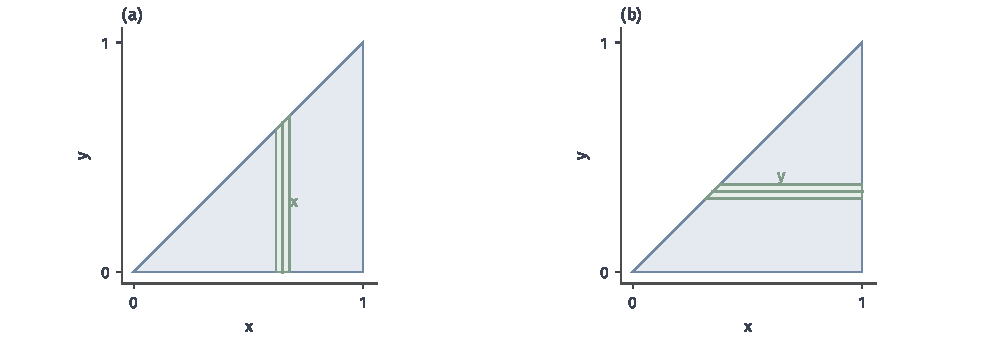
\includegraphics[width=169.0mm]{figures/01-mathematical-preliminaries-upper/01-mathematical-language-combinatorics-analysis-optimization/matplotlib/chapter3-concept-processes/region-slicing-orders.pdf}
 \caption{$D=\{0\leq y\leq x\leq1\}$在两图完全相同。(a) 固定$x$，纵截面为$0\leq y\leq x$；(b) 固定$y$，横截面为$y\leq x\leq1$。绿色窄条仅示意一次切片，图中的条宽不充当实际微元。两种累计$1$都得面积$1/2$；换序依据非负性或绝对可积性，而非图形本身。}
 \label{fig:analysis-process-region-slicing-orders}
\end{figure*}

\subsubsection{积分换序的适用边界}

这里非负性允许无穷值，绝对可积性则排除了依赖积分次序的条件相消。例如在
$\mathbb{N}\times\mathbb{N}$上使用计数测度时，Tonelli说明非负双重级数可以任意交换
求和次序；Fubini说明绝对收敛的双重级数也可以这样做。若既不非负也不绝对可积，
交换次序可能改变结果，甚至一个次序收敛而另一个发散。因此交换积分次序
需要先核对函数的非负性或绝对可积性。

\begin{example}[行列各自可加仍不足以换序]
\label{ex:analysis-iterated-sum-failure}
在正整数索引集$\{1,2,\ldots\}^2$上令
$a_{i,j}=\mathbb I\{j=i\}-\mathbb I\{j=i+1\}$，两边均用计数测度。
每一行只有一个$1$和一个$-1$，故$\sum_j a_{i,j}=0$；
第一列的和为$1$，其余每一列的和为$0$。于是
\[
 \sum_{i=1}^{\infty}\left(\sum_{j=1}^{\infty}a_{i,j}\right)=0,
 \qquad
 \sum_{j=1}^{\infty}\left(\sum_{i=1}^{\infty}a_{i,j}\right)=1.
\]
两种累次和都有有限值，却不相等。每行的绝对值和为$2$，所以整个绝对积分为无穷，
正负部分也各为无穷。失效的是Fubini的绝对可积条件，而非某一行的计算规则。
\end{example}


图~\ref{fig:vol1-add-fubini-cancellation-grid}显示这个例子的两条对角线。逐行的$+1$与$-1$配对，逐列的配对则从第二列才开始；无穷绝对和使这两种配对不能通过Fubini定理互换。
\begin{figure}[!htb]
  \centering
  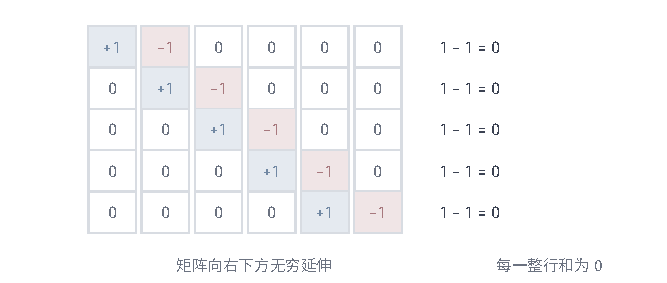
\includegraphics[width=112mm]{figures/01-mathematical-preliminaries-upper/01-mathematical-language-combinatorics-analysis-optimization/tikz/comprehension-additions/fubini-cancellation-grid.pdf}
  \caption{无穷矩阵$a_{i,j}=\mathbb I\{j=i\}-\mathbb I\{j=i+1\}$的左上角，展示前五行、前六列，矩阵向右下方继续。每一整行的和为$0$；第一整列的和为$1$，其他整列的和为$0$。蓝、红单元分别为$+1,-1$，每行绝对和为$2$，因而无穷矩阵不绝对可加。}
  \label{fig:vol1-add-fubini-cancellation-grid}
\end{figure}

$\sigma$有限也有实际作用。在$[0,1]$上让$x$采用Lebesgue测度、$y$采用
定义在所有子集上的计数测度，取非负函数$f(x,y)=\mathbb I\{x=y\}$。
对角线的补集是$[0,1]^2$内的相对开集；由前面欧氏开集的可数有理矩形表示，
它是可数个可测矩形的并。因此取补后，对角线属于乘积$\sigma$代数。
先对$y$计数再对$x$积分得到$1$，
先对$x$求长度再对$y$计数却得到$0$。这里不满足本章Tonelli版本的$\sigma$有限条件，
不能只凭非负性换序。

前面一元积分中的单调收敛、Fatou引理与支配收敛也适用于多维测度空间，因为证明使用简单函数和一般积分性质，并不依赖输入只有一个坐标。

\subsection{区域积分的换元}
\label{sec:multivariable-change-variables}

累次积分保留原坐标，只改变累计次序。换元则用一个向量值映射$T$同时改变位置的坐标表示，因此既要改写标量函数，也要校正每小块的体积。

\subsubsection{换元公式与适用条件}

\paragraph{体积的局部缩放}

一元换元用导数把参数增量换成长度增量；多元换元要把参数小块换成体积。
对方阵$\bm A$，$|\det\bm A|$是其线性映射对体积的放大倍数。
二维中，两列向量张成的平行四边形面积为$|\det\bm A|$；对角缩放$\operatorname{diag}(a_1,\ldots,a_d)$的比例为$\prod_j|a_j|$。
绝对值使方向反转后普通体积仍非负。

若$T$可微，Jacobian矩阵$\bm J_T(\bm x)$给出一点附近的线性近似，因此局部体积权重应是$|\det\bm J_T(\bm x)|$。
这个局部说明还不是整个积分公式的证明：整体上还必须控制近似误差，并确保参数化不会在正体积区域重复覆盖。

\paragraph{勒贝格积分的换元}

使用开集之间的$C^1$微分同胚，可以同时保证局部体积规则和全局单次覆盖。下面直接给出勒贝格版本，连续被积函数只是其中的一个特例。
\begin{theorem}[区域积分的换元公式]
设$U,V\subseteq\mathbb R^d$为开集，$T:U\to V$为$C^1$双射，逆映射也为$C^1$，且$\det\bm J_T$处处非零。
对任意非负勒贝格可测函数$g:V\to[0,\infty]$，有
\begin{equation}
 \int_Vg(\bm y)\,\mathrm d\bm y
 =\int_Ug(T(\bm x))|\det\bm J_T(\bm x)|\,\mathrm d\bm x,
 \label{eq:measurable-change-variables}
\end{equation}
允许共同值为$+\infty$。若$g$有符号且在$V$上绝对可积，则变换后的函数也绝对可积，等式仍成立并取有限值。
\end{theorem}

这类变换及其逆在局部紧邻域上是Lipschitz映射，因而保持零测集为零测集；结合Borel可测性，才能处理勒贝格完备化增加的集合。
一般定理先建立可测集合的体积变换，再从指示函数进入简单函数，最后以单调逼近得到非负函数的公式；有符号情形对$|g|$、$g^+$和$g^-$分别应用非负结论即可。
这里说明证明的依赖关系，集合层的体积变换定理引用测度论教材\scite{math-folland1999real}，不把逐点线性化当作完整证明。

若只在可测子区域$D\subseteq U$上积分，对$V$中的函数$g\mathbb I_{T(D)}$应用同一公式，即得
\begin{equation}
 \int_{T(D)}g(\bm y)\,\mathrm d\bm y
 =\int_Dg(T(\bm x))|\det\bm J_T(\bm x)|\,\mathrm d\bm x.
 \label{eq:analysis-multivariate-change-variables}
\end{equation}
这里不另加有界或边界零测的要求；所需条件仍是非负可测，或者有符号且绝对可积。
若参数化只在去掉零测边界或接缝以后为微分同胚，可以先在该范围内换元，再补回零测集。
若在正测度区域重复覆盖，则不能直接使用这个单次覆盖版本。

\subsubsection{常用坐标变换}

\paragraph{极坐标}

圆盘的边界用直角坐标描述时，积分上下限会含平方根。以半径和角度作为坐标，区域变成参数矩形，但面积权重必须增加半径因子。
\begin{example}[极坐标中的面积权重]
\label{ex:analysis-polar-coordinate-jacobian}
令$D=\{\bm{x}\in\mathbb{R}^2:\lVert\bm{x}\rVert_2\leq1\}$，并令
$T(r,\theta)=(r\cos\theta,r\sin\theta)$。在开集
$(0,1)\times(0,2\pi)$上，$T$是到开圆盘内部去掉原点和正$x$轴径向接缝后的区域的
连续可微双射，逆映射也连续可微。其Jacobian矩阵的行列式为
\[   \det
\begin{bmatrix}     \cos\theta & -r\sin\theta\\     \sin\theta & r\cos\theta
\end{bmatrix}   =r. \]
为了避开原点和接缝，可先限制$\varepsilon\leq r\leq1-\varepsilon$、$\varepsilon\leq\theta\leq2\pi-\varepsilon$，在每个这样的闭矩形上使用换元公式。遗漏的中心小圆盘、外侧窄环与接缝窄扇形面积随$\varepsilon\downarrow0$趋零；对有界被积函数，它们的累计贡献也趋零。因此取极限得到
\[   \int_D1\,\mathrm{d}\bm{x}   =   \int_0^{2\pi}\int_0^1r\,\mathrm{d}r\,\mathrm{d}\theta   =\pi. \]
这里积分上下限包含端点不改变积分值。若参数化在一片有正面积或体积的区域上重复覆盖，则不能直接使用
上述双射版本，否则同一点会被重复计数。
\end{example}

图~\ref{fig:vol1-add-polar-area-weight}说明半径因子来自哪里。同样的角度变化在较大半径处扫过更长的弧，故同样大小的参数块对应更大的面积，积分权重必须随半径变化。
\begin{figure}[!htb]
  \centering
  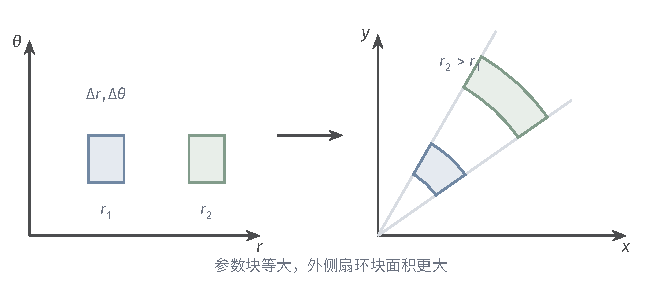
\includegraphics[width=112mm]{figures/01-mathematical-preliminaries-upper/01-mathematical-language-combinatorics-analysis-optimization/tikz/comprehension-additions/polar-area-weight.pdf}
  \caption{极坐标映射中的两个等大参数块，具有相同的$\Delta r,\Delta\theta$，但外侧半径$r_2$较大。对应扇环块的精确面积为$(r\Delta r+(\Delta r)^2/2)\Delta\theta$，一阶项为$r\Delta r\Delta\theta$，因此面积元为$r\,\mathrm dr\,\mathrm d\theta$。图只比较局部块，坐标原点与接缝的处理见正文。}
  \label{fig:vol1-add-polar-area-weight}
\end{figure}



\paragraph{柱坐标}

在三维中，柱坐标变换为$(x,y,z)=(r\cos\theta,r\sin\theta,z)$，体积元是$r\,\mathrm dr\,\mathrm d\theta\,\mathrm dz$。
例如半径$R$、高度$H$的圆柱体体积为
\[
 \int_0^H\int_0^{2\pi}\int_0^R r\,\mathrm dr\,\mathrm d\theta\,\mathrm dz=\pi R^2H.
\]
\paragraph{球坐标}

球坐标用到原点的距离$\rho$、从正$z$轴量起的夹角$\varphi$和绕$z$轴的角$\theta$：
\[
 (x,y,z)=(\rho\sin\varphi\cos\theta,\rho\sin\varphi\sin\theta,\rho\cos\varphi).
\]
其Jacobian行列式的绝对值为$\rho^2\sin\varphi$，故体积元为$\rho^2\sin\varphi\,\mathrm d\rho\,\mathrm d\varphi\,\mathrm d\theta$。
半径$R$的球由$0\leq\rho\leq R$、$0\leq\varphi\leq\pi$、$0\leq\theta\leq2\pi$描述，体积为
\[
 \int_0^{2\pi}\int_0^\pi\int_0^R\rho^2\sin\varphi\,\mathrm d\rho\,\mathrm d\varphi\,\mathrm d\theta
 =\frac{4\pi R^3}{3}.
\]
这里和极坐标一样，在内部单次覆盖处使用换元公式；坐标轴、原点及接缝的零测遗漏用极限补回。

\subsection{参数积分}
\label{sec:multivariable-parameter-integrals}

前面改变的是空间坐标。现在固定积分区域，让标量函数依赖一个实参数$\theta$，研究积分所得的数如何随这个参数变化；这分别涉及连续性、求导和端点变化三个问题。

\subsubsection{参数积分的定义}

设$(X,\mathcal A,\mu)$为测度空间，$I$为实参数区间，且对每个$\theta\in I$，$g(\cdot,\theta)$都是可积的标量函数。定义
\[
 G(\theta)=\int_Xg(x,\theta)\,\mathrm d\mu(x).
\]
固定参数后，$x$是被积变量；积分完成以后，$G$是一元参数函数。点态连续或点态可微只描述每个$x$处的变化，要将它们传递给$G$，还要控制整族函数的总贡献。

\subsubsection{参数积分的连续性}

参数趋近时，积分贡献可能集中到越来越小的区域，或移向无穷远。用同一个可积函数控制附近全部参数的贡献，可以通过支配收敛排除这些情况。
\begin{theorem}[可积控制下参数积分的连续性]
设$\theta_0\in I$，每个$g(\cdot,\theta)$可测。假设存在$\theta_0$在$I$中的一个相对邻域$J$、同一个可测零测集$N$及非负可积函数$h$，使对每个$x\notin N$，$g(x,\cdot)$在$\theta_0$连续，且
$|g(x,\theta)|\leq h(x)$对所有$\theta\in J$成立。
则$G(\theta)$在$J$上有有限值，并在$\theta_0$连续。
\end{theorem}
\begin{proof}
任取$\theta_n\to\theta_0$，充分大时$\theta_n\in J$。在$X\setminus N$上，$g(x,\theta_n)\to g(x,\theta_0)$，且绝对值都不超过$h(x)$。
支配收敛给出$G(\theta_n)\to G(\theta_0)$，由序列判据得到连续性。
\end{proof}

例如$g(x,\theta)=e^{-\theta x}$在$[0,\infty)$上积分，$\theta>0$时$G(\theta)=1/\theta$。
固定$\theta_0>0$，在其邻域内可由$e^{-\theta_0x/2}$支配，故$G$在$\theta_0$连续。控制函数只需覆盖所考察参数点的邻域，不要求同一上界适用于全部参数。

\subsubsection{积分号下求导}

积分号下求导实际要交换参数差商的极限与积分。各点偏导数存在只确定差商的点态极限；同一个可积函数控制全部差商，才足以将这个极限移入积分号。
\begin{theorem}[可积导数界下的积分号内求导]
固定$\theta_0$，设对每个$\theta\in I$，
$x\mapsto g(x,\theta)$可测，其中$I$是包含$\theta_0$的开区间，并且
$g(\cdot,\theta_0)$可积。假设存在一个可测零测集$N$，使每个$x\notin N$处的
$\theta\mapsto g(x,\theta)$在整个$I$内可微；对每个$\theta$，
偏导数作为$x$的函数可测，并且存在非负可积函数$h$使
\begin{equation}
  \left|
    \frac{\partial g}{\partial\theta}(x,\theta)
  \right|
  \leq h(x)
  \quad
  \text{对所有$x\notin N$及所有$\theta\in I$成立},
\label{eq:analysis-parameter-derivative-domination}
\end{equation}

则$I$内每个参数截面都可积，且
\begin{equation}
  G'(\theta_0)
  =
  \int_X
  \frac{\partial g}{\partial\theta}(x,\theta_0)
  \,\mathrm{d}\mu(x).
\label{eq:analysis-differentiate-under-integral}
\end{equation}
\end{theorem}
\begin{proof}
中值定理先给出
$|g(x,\theta)-g(x,\theta_0)|\leq|\theta-\theta_0|h(x)$，
所以$I$中每个$g(\cdot,\theta)$都可积，$G$在邻域内有有限值。
对非零$t$且$\theta_0+t\in I$，令
\[
 q_t(x)=\frac{g(x,\theta_0+t)-g(x,\theta_0)}{t}.
\]
中值定理又给出
\[
 |q_t(x)|\leq h(x)\qquad(x\notin N).
\]
差商在那里趋于$\partial g/\partial\theta(x,\theta_0)$。
对任意非零序列$t_n\to0$应用支配收敛，得到同一个积分极限；
由实数极限的序列判据，这就是$t\to0$的双侧极限。这正是所述导数公式。
\end{proof}

这里的零测集$N$和控制函数$h$都不能随参数改变。参数范围不可数，不能靠取全部参数例外集的并自动获得一个零测集。
条件~\eqref{eq:analysis-parameter-derivative-domination}是一组便于核对的充分条件；也可在更一般的版本中直接控制参数差商。

例如令$g(x,\theta)=e^{-\theta x}$，$x\in[0,\infty)$、$\theta>0$，
并用Lebesgue测度积分。固定$\theta_0>0$后取
$I=(\theta_0/2,3\theta_0/2)$，则
$|\partial_\theta g|=xe^{-\theta x}\leq xe^{-\theta_0x/2}=:h(x)$。
分部积分给出$\int_0^\infty h(x)\,\mathrm dx=4/\theta_0^2<\infty$，
没有需要删除的例外点，故
$G'(\theta_0)=-\int_0^\infty xe^{-\theta_0x}\,\mathrm dx=-1/\theta_0^2$，
与$G(\theta)=1/\theta$的直接求导一致。
若把参数范围放大到任意接近零的正数，便不能沿用这个固定的控制函数；
交换结论所需的是所考察参数点附近的统一控制。

\begin{example}[参数积分中的控制函数失效]
\label{ex:analysis-parameter-integral-failure}
下面考察参数域边界处对应的右求导问题。对$\theta\geq0$与$x\in(0,1)$，定义
\[   g(x,\theta)   =
\begin{cases}     \dfrac{\theta x}{x^2+\theta^2}, & \theta>0,\\[5pt]     0, & \theta=0.
\end{cases} \]
在$\theta=0$处，对每个固定$x>0$，关于$\theta$的右偏导数都等于$1/x$，但$1/x$在$(0,1)$上不可积。
直接积分得到
\[   G(\theta)   =   \frac{\theta}{2}   \log\left(\frac{1+\theta^2}{\theta^2}\right)   \quad(\theta>0),   \qquad G(0)=0. \]
于是$G(\theta)/\theta$在$\theta\downarrow0$时发散，$G$在$0$处没有有限右导数。积分内的
逐点右导数虽然存在，却缺少统一可积控制；因此这里不能交换右求导与积分。
\end{example}

\subsubsection{变限积分的求导}

前面的差商固定了积分区域。如果端点也变化，即使被积函数不依赖参数，积分仍然会变化。例如$G(\theta)=\int_0^\theta1\,\mathrm dx=\theta$的导数为一，只计算被积函数的参数偏导会遗漏这一贡献。
连续性能够逐点确定端点处的函数值，并将区间长度的变化转为边界贡献。
\begin{theorem}[变限参数积分的求导]
设$a(\theta),b(\theta)$在$\theta_0$附近可微，且$a(\theta)<b(\theta)$。
若$g(x,\theta)$和$\partial_\theta g(x,\theta)$在包含这些邻近积分区间的一个紧矩形上连续，则
\begin{equation}
 \begin{aligned}
 \frac{\mathrm d}{\mathrm d\theta}\int_{a(\theta)}^{b(\theta)}g(x,\theta)\,\mathrm dx
 &=\int_{a(\theta)}^{b(\theta)}\partial_\theta g(x,\theta)\,\mathrm dx\\
 &\quad+g(b(\theta),\theta)b'(\theta)
 -g(a(\theta),\theta)a'(\theta).
 \end{aligned}
\label{eq:measurable-moving-boundary-integral}
\end{equation}
\end{theorem}
\begin{proof}
记$a_0=a(\theta_0)$、$b_0=b(\theta_0)$。积分差可分解为
\[
 \begin{aligned}
 G(\theta)-G(\theta_0)
 &=\int_{a_0}^{b_0}\bigl[g(x,\theta)-g(x,\theta_0)\bigr]\,\mathrm dx\\
 &\quad+\int_{b_0}^{b(\theta)}g(x,\theta)\,\mathrm dx
 -\int_{a_0}^{a(\theta)}g(x,\theta)\,\mathrm dx.
 \end{aligned}
\]
短区间积分按端点次序采用有向约定。第一项除以$\theta-\theta_0$后，由固定区间内的积分号下求导趋于$\int_{a_0}^{b_0}\partial_\theta g(x,\theta_0)\,\mathrm dx$。
连续性使第二项等于
$g(b_0,\theta_0)[b(\theta)-b_0]+o(|b(\theta)-b_0|)$。端点的可微性保证$|b(\theta)-b_0|=O(|\theta-\theta_0|)$，所以它的差商趋于$g(b_0,\theta_0)b'(\theta_0)$。
第三项同理，并保留前面的负号，得到下端点贡献。三项相加即得公式。
\end{proof}

采用紧矩形上的连续性，是一组便于核对的充分条件。对一般可测函数，端点值还需有相应的取值与极限意义，不能仅凭几乎处处等价类任意指定边界读数。

\FloatBarrier
